The objective of the control module is to be capable of, with an input reference velocity and steering angle, outputting the appropriate command variables to achieve said references. The first step in its design is to conceptualize the car's model; since the interest lies in the motion of the car, the kinematic model will be the one to be studied.
\subsubsection{Conception Of Car Model}
\label{sec:concep}

\begin{figure}[!htbp]
\centering
       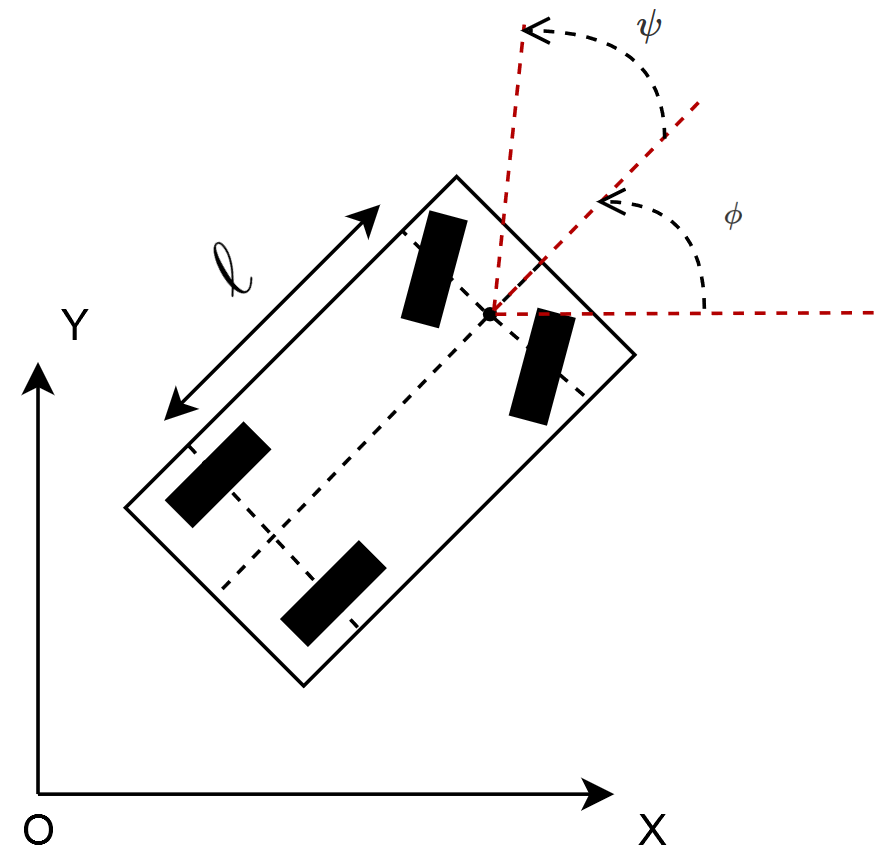
\includegraphics[page=1,width=0.6\textwidth]{img/kinematicModel.png} 
\caption{Kinematic Model of Car}%
\label{fig:kinModel}
\end{figure}

Considering the kinematic model of a four-wheel vehicle with a wheelbase length \gls{ell}, a linear velocity $v(t)$ and an angular velocity \gls{omega}$(t)$ the following situation will occur: since the rear wheels will remain in the same position no matter where the car is facing towards, they will be facing whatever orientation, \gls{phi}, the car is facing, however, in order for the car to be capable of moving into wherever the user tells it to, the front wheels must turn, ergo a steering angle \gls{psi}, must be considered. The resulting direction the car will be going in is $\phi + \psi$. With these considerations, a desired angle of tilt \gls{theta} and considering that $\phi=0$, in other words, that whatever direction the car is told to face, it will be relative to its current direction, the following model is obtained:
\begin{align}
\dot{x}&=v(t) cos(\psi)\\
\dot{y}&=v(t) sin(\psi)\\
\dot{\psi}&=\omega(t)=\frac{v(t)}{\ell}\theta
\end{align}
However this model is not enough for simulation purposes. The simulation has the objective of granting the designers clear ideas of the response of the systems towards given inputs, therefore, for implementation purposes, the simulation must give feedback on the position of the car, its heading and the linear velocity of the right rear wheel ($v_r$), and the left rear wheel ($v_l$) therefore the model will have to changed with these details in mind, which can be achieved considering that:
\begin{align}
\omega(t)&=\frac{v_r(t)-v_l(t)}{\ell}\\
v(t)&=\frac{1}{2}(v_r(t)+v_l(t))
\end{align}
Solving the system above for $v_r$ and $v_l$:
\begin{align}
v_ r(t)&=v(t)+ \frac{\omega(t)\ell}{2}\\
v_l(t)&=v(t)-\frac{\omega(t)\ell}{2}
\end{align}
Returning the model in order to $\dot{x}$ and $ \dot{y}$:
\begin{align}
\dot{x}&=v(t) cos(\psi)-\frac{\ell}{2}\omega(t) sin(\psi)\\
\dot{y}&=v(t) sin(\psi)+\frac{\ell}{2}\omega(t) cos(\psi)\\
\dot{\psi}&=\omega(t)=\frac{v(t)}{\ell}\theta
\label{equ:sysModel}
\end{align}
\subsubsection{Simulation Model}
The mathematical model determined in Section~\ref{sec:concep} was simulated in
the Matlab/Simulink environment. Converting the mathematical model into a
simulink subsystem yields (Fig.~\ref{fig:carModel}):
\begin{figure}[!htbp]
\centering
       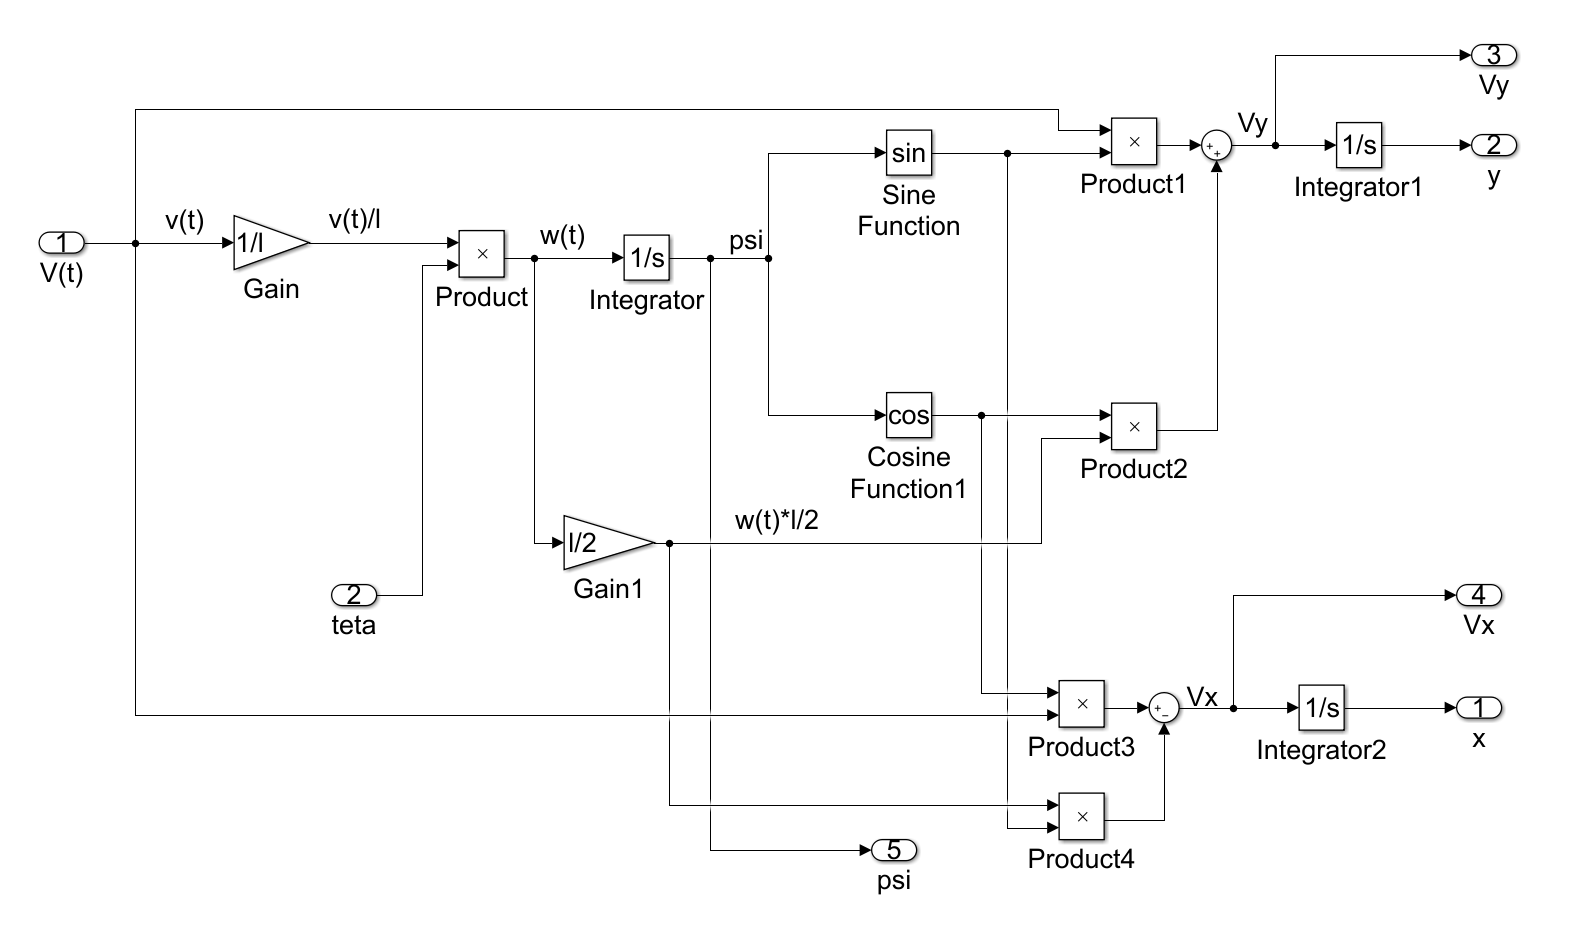
\includegraphics[page=1,width=1\textwidth]{img/subsystem.png} 
\caption{Car Model in a Simulink Subsystem}
\label{fig:carModel}
\end{figure}
The objective of the control module is making sure that the linear velocities of the right and left wheels achieve the desired values, consequently controlling the linear velocity of the rover and its steering angle. Therefore that is what the simulation model takes into account, two controllers, one for each, wheel will make sure that both the steeting angle and the linear velocity reach the desired values. This results in the schematic obtained in Fig.~\ref{fig:simSche}.
\begin{figure}[!htbp]
\centering
       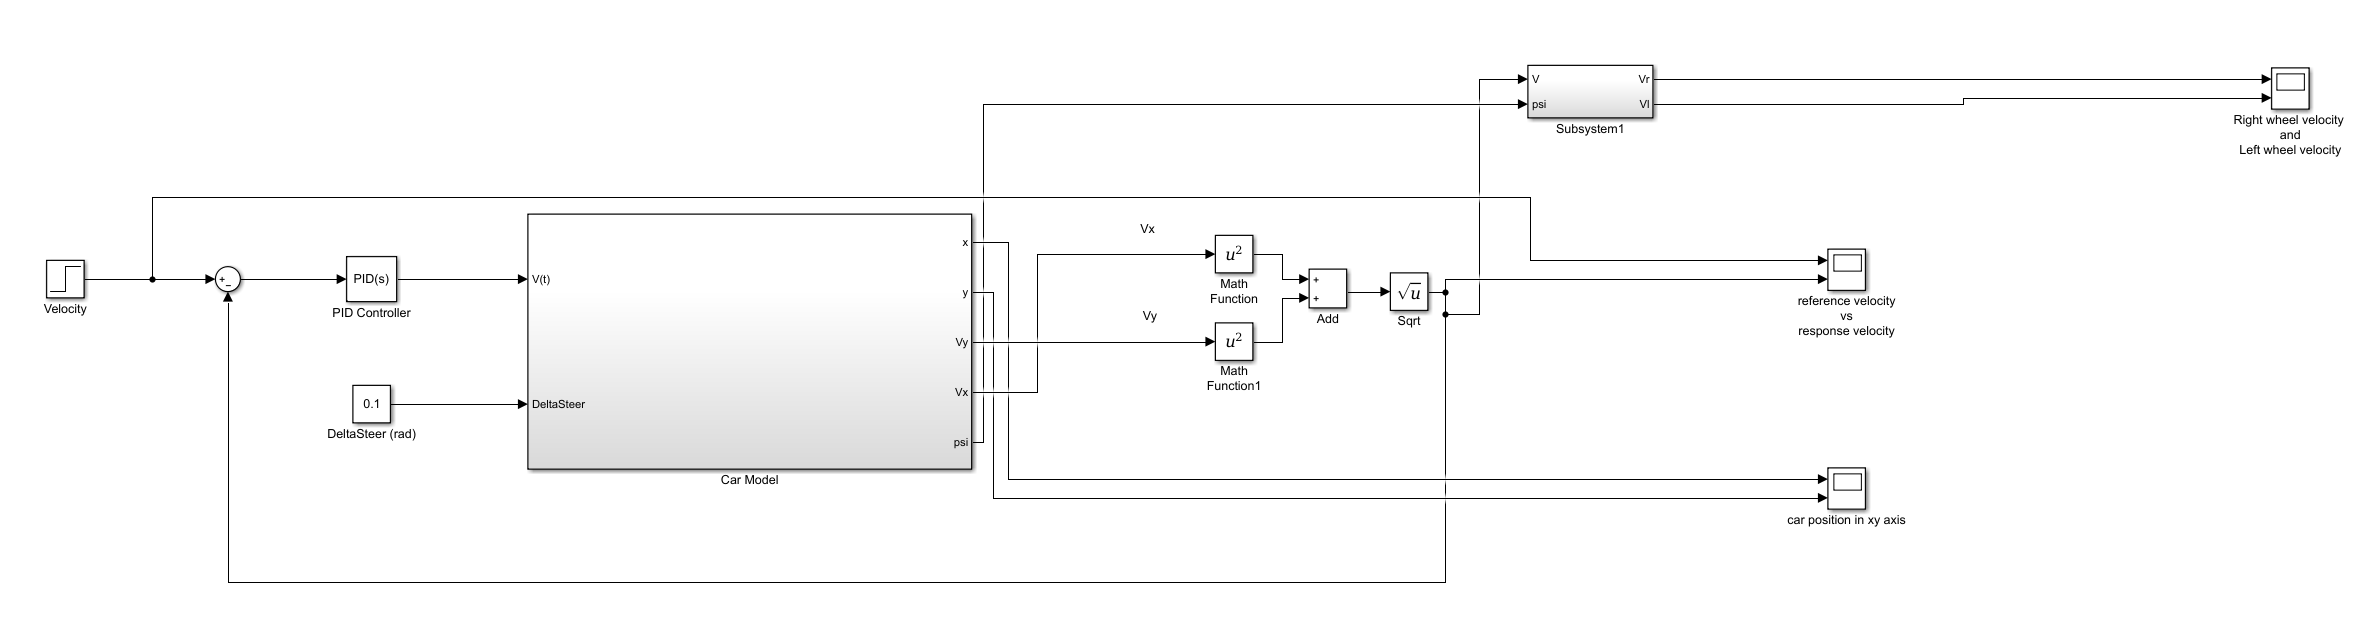
\includegraphics[page=1,width=1\textwidth]{img/system.png} 
\caption{Simulation Schematic}
\label{fig:simSche}
\end{figure}\\